\documentclass[11pt,a4paper,oneside]{report}
\usepackage[T1]{fontenc}
\usepackage[utf8]{inputenc}
\usepackage[french]{babel}
\usepackage{lmodern}
\usepackage[a4paper,margin=2.5cm,headheight=15pt]{geometry}
\usepackage{microtype}
\usepackage{graphicx}
\usepackage{float}
\usepackage{xcolor}
\usepackage{booktabs,tabularx,array}
\usepackage{enumitem}
\usepackage{fancyhdr}
\usepackage{titlesec}
\usepackage{hyperref}
\definecolor{bleunuit}{HTML}{12304A}
\definecolor{bleuclair}{HTML}{2C668A}
\hypersetup{colorlinks=false,pageanchor=false,pdftitle={Rapport de tests — Éditeur collaboratif},pdfsubject={Validation fonctionnelle et mesures locales}}
\setlength{\parindent}{0pt}
\setlength{\parskip}{6pt}
\setlist{nosep,leftmargin=*}
\pagestyle{fancy}
\fancyhf{}
\fancyhead[L]{\small Rapport de tests}
\fancyhead[R]{\small Éditeur collaboratif}
\fancyfoot[C]{\thepage}
\renewcommand{\headrulewidth}{0.4pt}
\titleformat{\chapter}{\normalfont\huge\bfseries}{\thechapter}{1em}{}
\titleformat{\section}{\normalfont\Large\bfseries}{\thesection}{1em}{}

\begin{document}
\begin{titlepage}
\pagecolor{bleunuit}\color{white}
\thispagestyle{empty}
\vspace*{1.2cm}
{\Large UNIVERSITÉ DE YAOUNDÉ I\par}
\vspace{.2cm}
{\large École Nationale Supérieure Polytechnique de Yaoundé\\Département de Génie Informatique\par}
\vfill
\color{white}\rule{\textwidth}{1.2pt}\par
\vspace{1.0cm}
{\Huge\bfseries Rapport de tests\par}
\vspace{.5cm}
{\LARGE Éditeur collaboratif de documents\par}
\vspace{.4cm}
{\large Tests fonctionnels, cohérence et mesures de charge locales\par}
\vspace{1.0cm}
\color{white}\rule{\textwidth}{1.2pt}\par
\vfill
\begin{tabular}{@{}ll@{}}
Étudiant : & OSSOMBE Pierre René Raoul\\
Formation : & Génie informatique — 5\textsuperscript{e} année\\
Encadrement : & Pr Jean Marc Menaud\\
Date de campagne : & 26 octobre 2026
\end{tabular}
\vspace{1.2cm}
\end{titlepage}
\nopagecolor\color{black}
\hypersetup{pageanchor=true}
\pagenumbering{roman}
\chapter*{Résumé exécutif}
La campagne confirme le bon fonctionnement des principaux contrôles métier sur l’environnement local : les trois tests d’intégration passent, la compilation de l’API et de l’interface réussit, les 300 connexions WebSocket testées reçoivent leur état initial, et un PDF généré a été téléchargé et reconnu comme fichier PDF valide.

Les mesures HTTP portent sur des lectures locales et ne représentent pas le parcours complet de 15\,000 visiteurs. Les 300 connexions WebSocket provenaient d’un seul compte de test. La capacité exigée de 15\,000 visiteurs, dont 12\,000 dans la première minute, avec 300 rédacteurs actifs, reste donc à démontrer sur l’infrastructure cible. Ce rapport ne revendique pas cette capacité.

\tableofcontents
\clearpage
\pagenumbering{arabic}

\chapter{Objet et périmètre}
Ce rapport consigne les vérifications réalisées sur l’application de rédaction collaborative. La campagne couvre les tests d’intégration existants, la compilation, des lectures HTTP concurrentes, l’ouverture de connexions WebSocket et un téléchargement PDF de bout en bout.

Les essais ont été exécutés le 26 octobre 2026 sur l’environnement local de développement. L’API répondait sur le port 3000 et PostgreSQL 16.15 sur le port 5433. La machine de test disposait de 16 processeurs logiques et d’environ 15 Gio de mémoire visible. Node.js 22.22.0 et npm 10.9.4 étaient installés. Aucune campagne AWS n’a été exécutée.

\section{Précautions de campagne}
Les scénarios de charge HTTP interrogent des routes de lecture. Le test PDF a consommé une seule utilisation d’un lien créé pour l’essai. Le test de 300 connexions WebSocket n’a envoyé aucune édition massive. Ces précautions évitent de créer une file de milliers de travaux PDF dans l’environnement de développement.

\chapter{Méthode et critères}
Les tests d’intégration utilisent la suite Node.js du dépôt et une base PostgreSQL locale. Les mesures HTTP utilisent 40 requêtes simultanées pour chaque scénario, avec 1\,000 requêtes au total. Les latences sont calculées côté générateur, du début de la requête à la lecture complète de la réponse. Les percentiles sont les valeurs observées aux rangs p50, p95 et p99.

Le test WebSocket ouvre 300 connexions vers le même document et attend le message initial de synchronisation sur chaque connexion. Le parcours PDF crée un compte de test, un document, une sauvegarde, un lien limité, réserve une utilisation, attend l’état prêt et télécharge le fichier. La validité minimale du PDF est contrôlée par sa signature binaire « \texttt{\%PDF-} ».

\chapter{Résultats}
\section{Compilation et tests d’intégration}
La commande \texttt{npm run build} a compilé l’API TypeScript et l’interface Vite sans erreur. La suite \texttt{npm test} a migré le schéma puis exécuté trois tests :
\begin{itemize}
  \item fusion d’éditions Yjs simultanées, persistance et diffusion de présence ;
  \item respect exact du quota de lien sous 40 réservations concurrentes, idempotence, épuisement et calcul du crédit partagé ;
  \item contrôle des sessions, des rôles et des opérations d’administration.
\end{itemize}

\begin{center}
\begin{tabular}{@{}lrr@{}}
\toprule
Résultat & Nombre & Statut\\
\midrule
Tests réussis & 3 & Réussi\\
Tests échoués & 0 & Réussi\\
Tests ignorés & 0 & Réussi\\
\bottomrule
\end{tabular}
\end{center}
La sortie TAP complète est conservée dans \texttt{preuves/integration.tap.log}.

\section{Lectures HTTP concurrentes}
Les deux routes ont répondu avec le code HTTP 200 pour les 1\,000 requêtes de chaque scénario.

\begin{center}
\small
\begin{tabularx}{\textwidth}{@{}Xrrrrr@{}}
\toprule
Scénario & Requêtes & Concurrence & Débit (req/s) & p95 (ms) & p99 (ms)\\
\midrule
État de santé \texttt{/health} & 1\,000 & 40 & 1\,533.2 & 67.1 & 103.1\\
Lecture publique d’un lien & 1\,000 & 40 & 2\,275.2 & 25.0 & 26.8\\
\bottomrule
\end{tabularx}
\end{center}

Pour \texttt{/health}, le temps total était de 652.3 ms et la latence p50 de 20.9 ms. Pour la lecture publique, le temps total était de 439.5 ms et la latence p50 de 16.8 ms. Toutes les réponses étaient HTTP 200. Les résultats bruts et le script de reproduction sont fournis dans \texttt{preuves/charge-locale.json} et \texttt{outils/charge-locale.mjs}. Ces résultats décrivent des lectures sur une instance locale; ils ne prédisent pas le débit AWS ni celui d’opérations d’écriture.

\section{Connexions WebSocket}
Sur 300 connexions ouvertes simultanément vers un document, 300 messages de synchronisation initiaux ont été reçus et aucune connexion n’a échoué. L’ouverture complète a pris 827.8 ms, soit 362.4 connexions par seconde. Les latences d’ouverture mesurées étaient p50 = 311.0 ms, p95 = 742.7 ms et p99 = 791.6 ms. La sortie JSON complète est conservée dans \texttt{preuves/charge-locale.json}.

Les 300 sessions utilisaient le même compte de test. Cet essai valide une charge de connexions sur un processus local, mais ne valide pas 300 identités, l’activité continue de 300 éditeurs, la convergence sous édition soutenue ni une architecture multi-instance.

\section{Réservation et fichier PDF}
Une réservation a reçu HTTP 202, a atteint l’état \texttt{READY} à la révision 1, puis le téléchargement a répondu HTTP 200. Le fichier téléchargé faisait 1\,576 octets et commençait par la signature attendue \texttt{\%PDF-}. Le parcours a pris 511.6 ms entre la première interrogation du statut et le téléchargement. Une seule unité de quota a été consommée. La preuve structurée est conservée dans \texttt{preuves/pdf-e2e.json}.

\chapter{Analyse et limites}
Les résultats confirment les propriétés couvertes par les scénarios exécutés : les invariants de quota et de crédit sous les concurrences ciblées par les tests d’intégration, les contrôles d’accès, le démarrage WebSocket simultané et la génération d’un PDF téléchargeable.

Ils ne démontrent pas les objectifs de charge du cahier des charges. En particulier, aucun essai n’a envoyé 15\,000 clics de visiteurs, dont 12\,000 dans la première minute, tout en maintenant 300 rédacteurs actifs. Le test WebSocket ne simule ni des identités distinctes ni des modifications répétées. L’environnement utilisé ne comprend pas de campagne de déploiement AWS instrumentée; S3, SQS, SES, l’équilibrage de charge, la montée en charge des API et des workers ne sont pas validés ici.

Une campagne complète doit être conduite sur un environnement isolé et dimensionné, avec des liens et documents dédiés. Elle devra enregistrer les résultats bruts, les latences p50/p95/p99, le débit, les erreurs fonctionnelles et réseau, la profondeur de file PDF, les ressources consommées, les journaux AWS et les coûts. Les critères d’acceptation doivent distinguer une réponse fonctionnelle (prêt, en attente ou quota épuisé) d’un refus technique ou d’un délai dépassé.

\chapter{Conclusion}
La validation locale est positive pour les scénarios fonctionnels exécutés et pour une charge modérée de lectures et de connexions WebSocket. La capacité cible du projet n’est pas encore prouvée. Le rapport devra être complété après une campagne de charge complète sur l’environnement de déploiement, sans remplacer les résultats mesurés par une extrapolation des tests locaux.

\appendix
\chapter{Reproduction des vérifications}
Depuis le dossier \texttt{application/}, avec PostgreSQL démarré sur le port configuré dans \texttt{.env} :
\begin{verbatim}
npm run build
npm test
\end{verbatim}
Les mesures HTTP et WebSocket consignées ici ont été exécutées avec \texttt{node '../Rapport de test/outils/charge-locale.mjs'} contre l’API locale sur \texttt{http://127.0.0.1:3000}. Le script crée un compte, un document et un lien de test; il ne réserve aucun téléchargement. Le parcours PDF dédié, reproductible avec \texttt{node '../Rapport de test/outils/pdf-e2e.mjs'}, consomme une unité de quota. Les journaux de preuve et leurs empreintes figurent dans \texttt{preuves/} et \texttt{preuves/SHA256SUMS}.

\chapter{Pièces justificatives}
Les fichiers suivants accompagnent ce rapport afin qu’un lecteur puisse vérifier les affirmations et répéter les essais :
\begin{itemize}
  \item \texttt{preuves/build.log} : sortie de compilation API et interface ;
  \item \texttt{preuves/integration.tap.log} : sortie TAP des tests d’intégration ;
  \item \texttt{preuves/charge-locale.json} : résultats bruts des deux charges HTTP et des 300 connexions WebSocket ;
  \item \texttt{preuves/pdf-e2e.json} : statuts HTTP, état final, révision, taille et signature du PDF ;
  \item \texttt{resultats-bruts.json} : résultats consolidés ; les scripts de reproduction sont dans \texttt{outils/}.
\end{itemize}
Les quatre images de \texttt{preuves/captures/} sont des rendus visuels en noir et blanc des sorties conservées, et non des captures directes de l’écran. Les journaux bruts restent les pièces de référence. Le fichier \texttt{preuves/SHA256SUMS} donne une empreinte SHA-256 des journaux et des images, afin de détecter une modification après génération. Ces pièces ne contiennent ni identifiants de session ni secrets de configuration.

\chapter{Captures visuelles des résultats}
Les figures ci-dessous facilitent la lecture des résultats. Chaque figure est dérivée d’un journal ou d’un résultat JSON identifié dans les légendes; le fichier source permet de vérifier les valeurs exactes.

\begin{figure}[H]
  \centering
  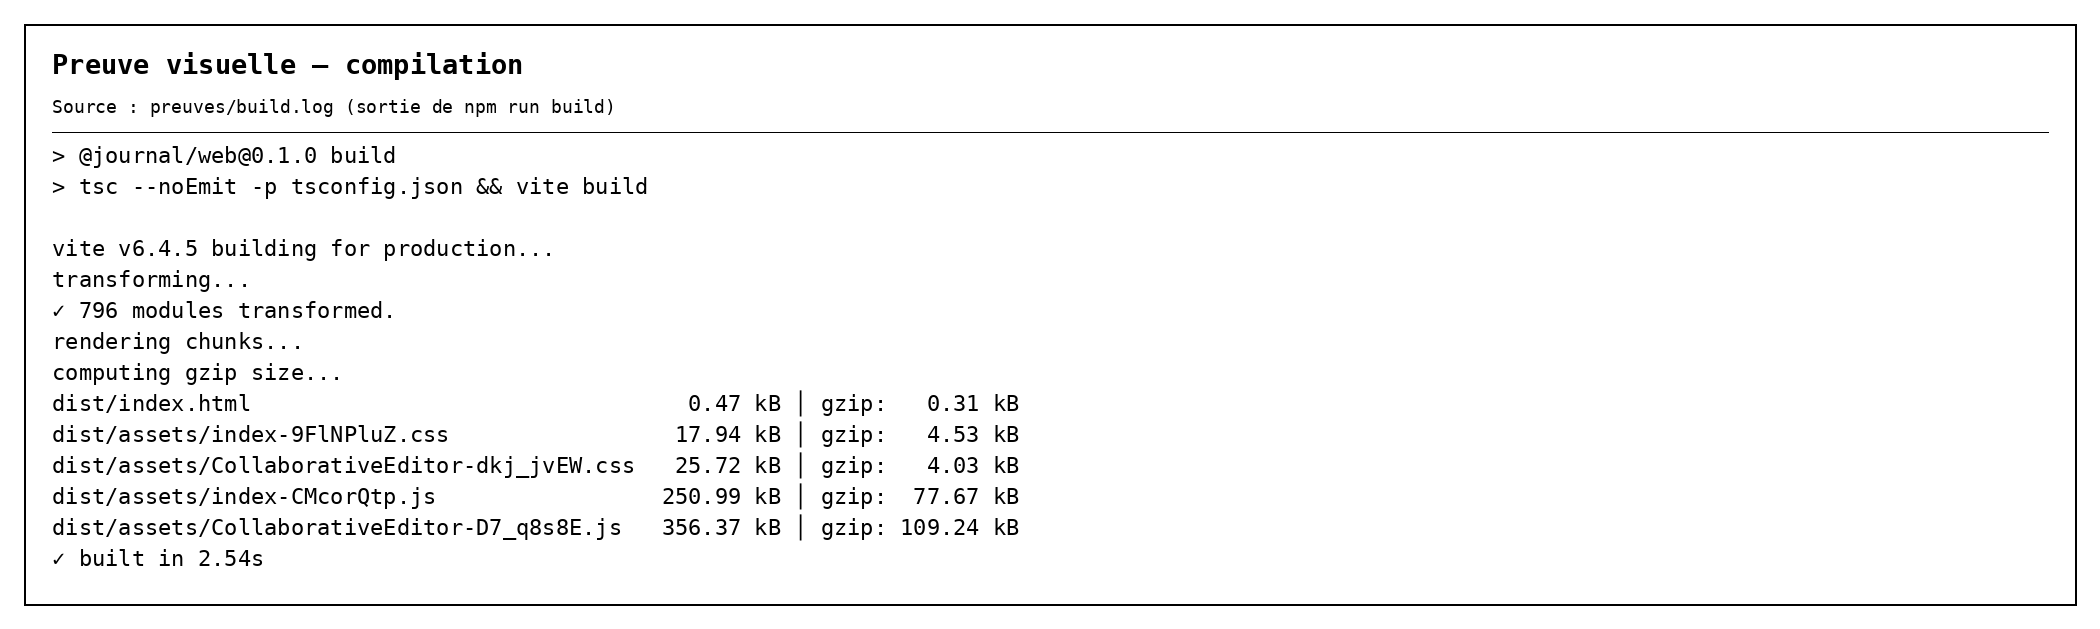
\includegraphics[width=\textwidth]{preuves/captures/compilation.png}
  \caption{Sortie de compilation de l’API et de l’interface.}
\end{figure}
\begin{figure}[H]
  \centering
  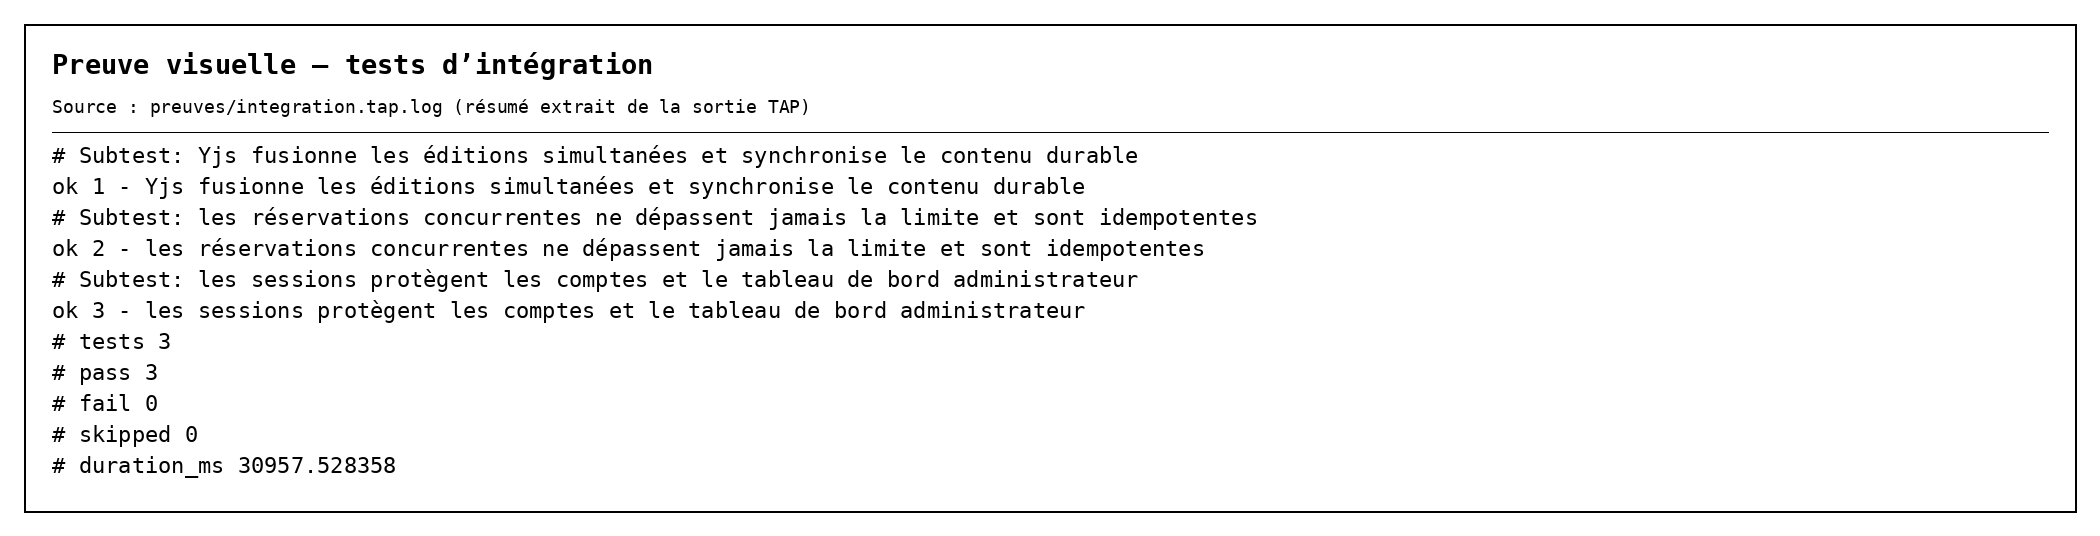
\includegraphics[width=\textwidth]{preuves/captures/integration.png}
  \caption{Sortie TAP des trois tests d’intégration réussis.}
\end{figure}
\clearpage
\begin{figure}[H]
  \centering
  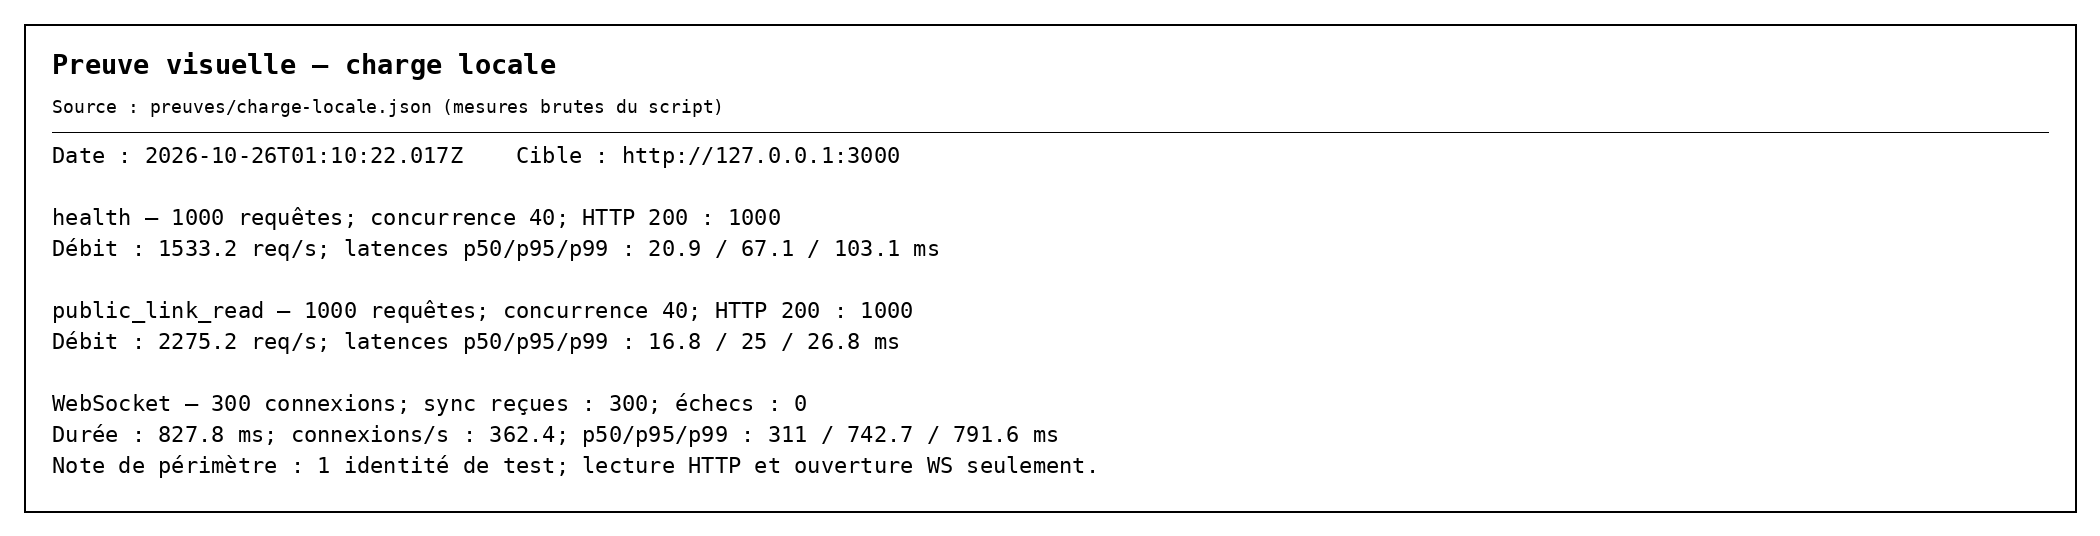
\includegraphics[width=\textwidth]{preuves/captures/charge-locale.png}
  \caption{Résumé visuel des mesures HTTP et des 300 synchronisations WebSocket locales.}
\end{figure}
\begin{figure}[H]
  \centering
  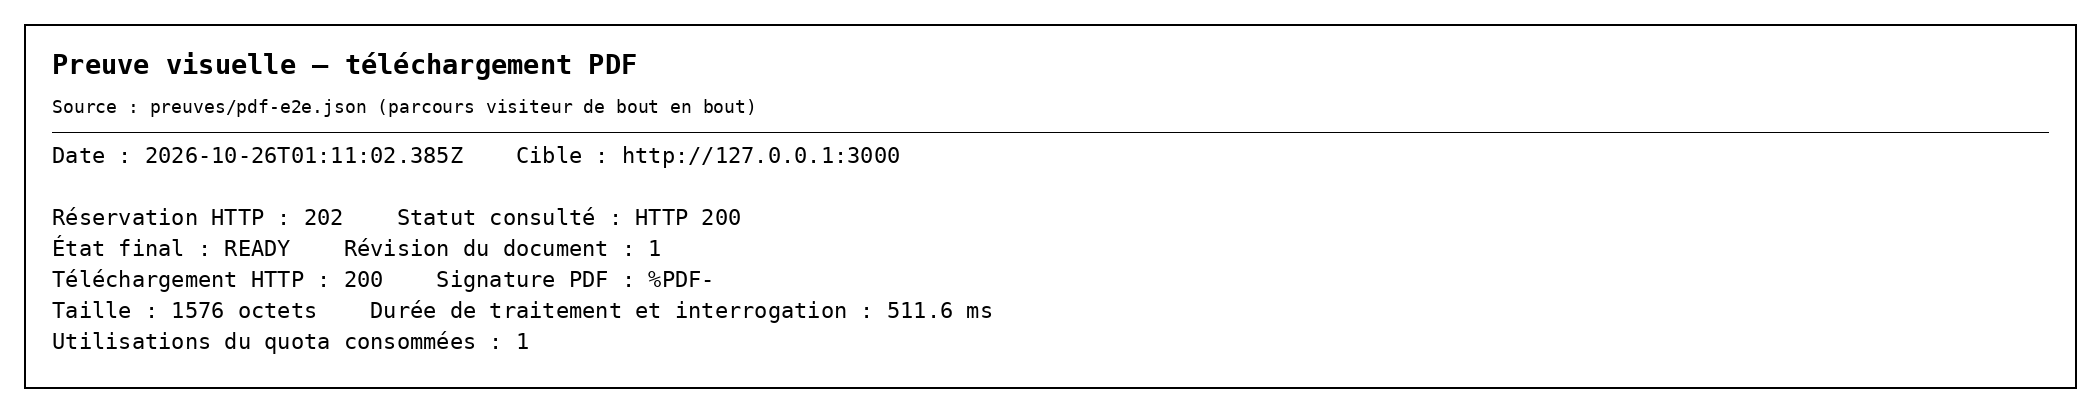
\includegraphics[width=\textwidth]{preuves/captures/pdf-e2e.png}
  \caption{Réservation visiteur et validation du fichier PDF téléchargé.}
\end{figure}

\chapter{Justificatif des coûts AWS}
Les essais de ce rapport ont été exécutés sur l’environnement local. Aucun déploiement AWS ni accès aux données de facturation AWS n’a été utilisé pendant cette campagne. Il n’est donc pas possible d’y joindre une capture authentique du coût AWS du projet; ce justificatif demeure à fournir.

Après le déploiement, joindre une capture de Cost Explorer montrant la période, la devise, les filtres et le regroupement par service, puis la page Bills ou la facture correspondante. Cost Explorer est utile pour analyser l’évolution et la répartition des coûts; la facture clôturée établit le montant final dû. Pour une période en cours, AWS indique que le montant est estimatif et que les données de facturation sont actualisées au moins quotidiennement. Voir la documentation AWS sur \href{https://docs.aws.amazon.com/awsaccountbilling/latest/aboutv2/getting-viewing-bill.html}{les factures} et \href{https://docs.aws.amazon.com/us_en/awsaccountbilling/latest/aboutv2/differences-billing-data-cost-explorer-data.html}{les différences entre les données Billing et Cost Explorer}.

Une capture de l’AWS Pricing Calculator peut compléter l’analyse en documentant le coût prévisionnel et ses hypothèses, mais elle ne remplace pas la preuve des frais réellement engagés. Masquer l’identifiant du compte, les coordonnées personnelles et toute information de paiement avant l’insertion.

\end{document}
